\documentclass{article}

\usepackage[utf8]{inputenc}
\usepackage[brazil]{babel}
\usepackage{amsmath}
\usepackage{amsfonts}
\usepackage[section]{placeins}
\usepackage{booktabs}
\usepackage{multirow}
\usepackage{listings}
\usepackage{booktabs}
\usepackage[title]{appendix}

\usepackage{caption}

\usepackage{hanging}
\usepackage{graphicx}

\usepackage{natbib}
\usepackage{float}

% Commands --------------------------------------------------------------------

\newcommand\indep{\protect\mathpalette{\protect\independenT}{\perp}}
\def\independenT#1#2{\mathrel{\rlap{$#1#2$}\mkern2mu{#1#2}}}

\setlength{\parskip}{0.5em}

\def\arraystretch{1.5}

% Document basics -------------------------------------------------------------

\title{Métodos Numéricos - Problem set 05}
\author{Samuel de S. Barbosa}
\date{June, 2018}

\begin{document}

\maketitle

In this problem set we will numerically solve a simple savings problem in a
economy with idiosyncratic shocks.

Suppose there is a continuum of goat farmers that are subject to endowment
shocks. A farmer's endowment is $e^z$, where $z$ follows the following
stochastic process:

$$z^\prime = \rho z + \epsilon,$$

where $\epsilon \sim N(0,\sigma^2)$. The farmers instantaneous utility
function is given by

$$u(c) = \frac{c^{1-\gamma}-1}{1-\gamma}$$

and he discounts the future with the factor $\beta \in (0,1)$. Each farmer has
access to a storage technology such that, if he sets aside q goats today, he
will have 1 goat tomorrow. His budget constraint can then be writte as:

$$c + qa^\prime = e^z + a$$

Let $\beta = q = 0.96$ and $\gamma = 1.0001$ for now.

\section*{1.a)}

Let $\rho = 0.9$ and $\sigma = 0.01$. Using the Tauchen method to discretize the
stochastic process in a Markov chain with 9 states, with 3 standard deviations
for each side, we have the following grid for $e^z$ and transition matrix

\begin{scriptsize}
\begin{tabular}{lllllllll}
   0.9335 &   0.9497  &  0.9662  &  0.9829  &  1.0000   & 1.0174 &   1.0350 &   1.0530  &  1.0712
\end{tabular}

P = \begin{bmatrix}
    0.5683 & 0.4025 & 0.0290 & 0.0002 & 0.0000 & 0.0000 &      0 &      0 &      0 \\[0.3em]
    0.0843 & 0.5503 & 0.3459 & 0.0194 & 0.0001 & 0.0000 & 0.0000 &      0 &      0 \\[0.3em]
    0.0017 & 0.1125 & 0.5829 & 0.2902 & 0.0126 & 0.0000 & 0.0000 & 0.0000 &      0 \\[0.3em]
    0.0000 & 0.0029 & 0.1480 & 0.6034 & 0.2376 & 0.0080 & 0.0000 & 0.0000 & 0.0000 \\[0.3em]
    0.0000 & 0.0000 & 0.0049 & 0.1899 & 0.6104 & 0.1899 & 0.0049 & 0.0000 & 0.0000 \\[0.3em]
    0.0000 & 0.0000 & 0.0000 & 0.0080 & 0.2376 & 0.6034 & 0.1480 & 0.0029 & 0.0000 \\[0.3em]
    0.0000 & 0.0000 & 0.0000 & 0.0000 & 0.0126 & 0.2902 & 0.5829 & 0.1125 & 0.0017 \\[0.3em]
    0.0000 & 0.0000 & 0.0000 & 0.0000 & 0.0001 & 0.0194 & 0.3459 & 0.5503 & 0.0843 \\[0.3em]
    0.0000 & 0.0000 & 0.0000 & 0.0000 & 0.0000 & 0.0002 & 0.0290 & 0.4025 & 0.5683 \\[0.3em]
\end{bmatrix}
\end{scriptsize}

\section*{1.b)}

Now we discretize the asset space using a grid starting from the natural debt limit under
the worst endowment state up to two times the savings under the best state. 
This gives us a grid in $[-23.3373, 53.5624]$, with 1.000 points.

Solving the individual goat farmer problem for each state variable, using vectorized
brute force on Matlab, we get the following value and policy functions:

\begin{figure}[H]
  \centering
    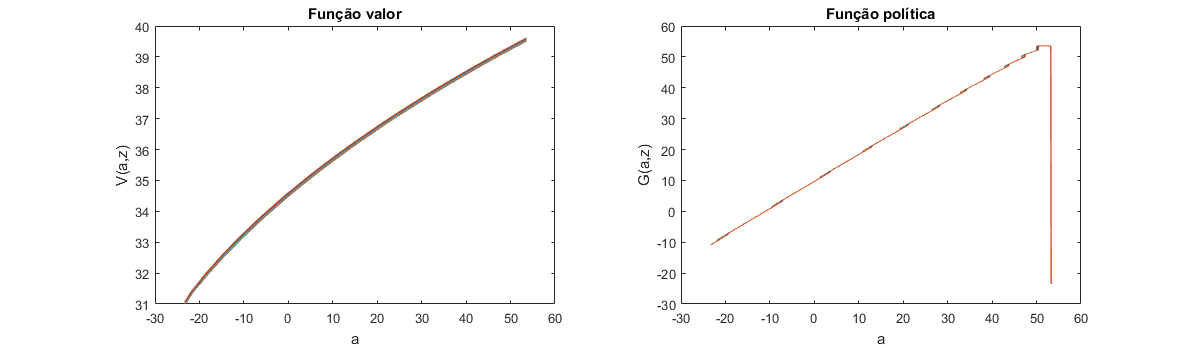
\includegraphics[width=\textwidth]{graf1.png}
\end{figure}

\section*{1.c)}

Next we find the stationary distribution $\pi(z, a)$ and use it to compute the aggregate savings in the
economy.

As we have a continuum of goat farmers in our economy, their stationary distribution over $a$ and $z$
will depend only on $\pi(z)$:

\begin{scriptsize}
\begin{tabular}{l|rrrrrrrrr}
   $e^z$  & -0.6170 & -0.4628 & -0.3085 & -0.1543 & 0.0000 &  0.1543  &  0.3085 &   0.4628 & 0.6170 \\ \hline
   $\pi(z)$ & 0.0073 &  0.0352 &  0.1089 &  0.2143 & 0.2685  &  0.2143  &  0.1089 &   0.0352 & 0.0073 \\
\end{tabular}
\end{scriptsize}

We then compute the aggregate savings from

	$$ A = \sum_a \sum_z \pi(a,z) a'(a,z) $$

which gives us an aggregate savings of 21.46.

\section*{1.d)}

Now we redo the analysis using $\rho = 0.97$. Our economy now presents more
variance of endowments over states (more variance in the grid of $e^z$) and it
also exhibits more persistence in states, as exhibited by the transition
matrix.

\begin{scriptsize}
\begin{tabular}{lllllllll}
   0.8839  &  0.9116 &   0.9402&    0.9696 &   1.0000 &   1.0313 &   1.0636 &   1.0970  &  1.1313
\end{tabular}

P = \begin{bmatrix}
    0.8795  &  0.1205  &  0.0000  &  0.0000  &       0  &       0  &       0  &       0  &       0 \\[0.3em]
    0.0344  &  0.8627  &  0.1029  &  0.0000  &  0.0000  &       0  &       0  &       0  &       0 \\[0.3em]
    0.0000  &  0.0420  &  0.8707  &  0.0873  &  0.0000  &  0.0000  &       0  &       0  &       0 \\[0.3em]
    0.0000  &  0.0000  &  0.0510  &  0.8755  &  0.0735  &  0.0000  &  0.0000  &       0  &       0 \\[0.3em]
    0.0000  &  0.0000  &  0.0000  &  0.0615  &  0.8771  &  0.0615  &  0.0000  &  0.0000  &       0 \\[0.3em]
    0.0000  &  0.0000  &  0.0000  &  0.0000  &  0.0735  &  0.8755  &  0.0510  &  0.0000  &  0.0000 \\[0.3em]
    0.0000  &  0.0000  &  0.0000  &  0.0000  &  0.0000  &  0.0873  &  0.8707  &  0.0420  &  0.0000 \\[0.3em]
    0.0000  &  0.0000  &  0.0000  &  0.0000  &  0.0000  &  0.0000  &  0.1029  &  0.8627  &  0.0344 \\[0.3em]
    0.0000  &  0.0000  &  0.0000  &  0.0000  &  0.0000  &  0.0000  &  0.0000  &  0.1205  &  0.8795 \\[0.3em]
\end{bmatrix}
\end{scriptsize}

Farmers now are exposed to more variance over endowments, and longer streaks
of the same type of endowment states. Thus, being in low endowment states
are now worse than before, and, on the other side, being on high states are
better. This gives us value functions that are more spread over states.

Since farmers are risk averse, they reduce this increased variance by
saving more. We now have an aggregate savings of 23.66.

\section*{1.e)}

If we suppose further that $\gamma = 5$, agents are now more risk averse than
before. They want more smooth consumption than before. As a result, they save
less under  low endowment sates and save more under high ones. Value functions
are thus more concave.

Aggregate savings actually drops to 19.78, because reduced savings under low
endowment states overwhelms increased savings under high states.

\section*{1.f)}

If we suppose $\sigma=0.05$, variance over endowment states get way larger.

\begin{scriptsize}
\begin{tabular}{lllllllll}
   0.5396  &  0.6295  &  0.7345  &  0.8571   & 1.0000 &   1.1668   & 1.3614   & 1.5885  &  1.8534
\end{tabular}
\end{scriptsize}

\end{document}
